\documentclass[12pt, a4paper]{article}
\usepackage{amsmath}
\usepackage{amsfonts}
\usepackage{amsthm}
\usepackage{mathtools}
\newtheorem{theorem}{Theorem}[section]
\newtheorem{definition}{Definition}[section]
\numberwithin{equation}{section}
\usepackage{pgfplots}
\pgfplotsset{width=10cm,compat=1.9}
\graphicspath{ {img/} }
\DeclareGraphicsExtensions{.png,.jpg}

\title{Support Vector Machines}
\author{Kristian Wichmann}

\begin{document}
\maketitle

\section{Overview}
At its heart, a \textit{support vector machine} (SVM) is a binary classifaction algorithm. The basic version creates a linear decision boundary, but using a strategy known as the \textit{kernel trick}, we can make SVM's produce non-linear decision boundaries.

\section{Linearly separable data}
Initially, we assume that the data can be perfectly classified by a linear decision boundary - a hyperplane in configuration space such that all positives are on one side and all negatives on the other side. Generally, this can be done in many ways. So we will specifically search for the one which maximizes the perpendicular distance to the closest data points. Such closest point are known as \textit{support vectors}. See figure \ref{fig:svm_linear}.

\begin{figure}
\centering
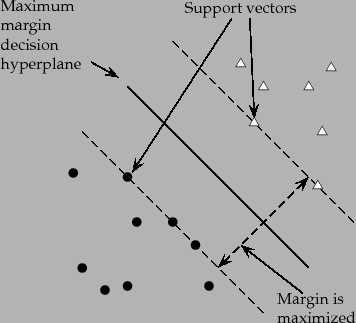
\includegraphics[scale=0.5]{svm1}
\caption{We're searching for the widest possible separation "road".}
\label{fig:svm_linear}
\end{figure}

\subsection{Classifying a new data point}
If we have a new data point $\vec{u}$, we might ask whether or not our algorithm classifies $\vec{u}$ as a positive or a negative.

The separation boundary is a hyperplane. Let $\vec{w}$ be a normal vector to this hyperplane\footnote{The chosen vector is sometimes referred to as the \textit{weight vector}.}. We want to know how far in the direction of $\vec{w}$ our new data point $\vec{u}$ goes. In other words, we want to know the projection of $\vec{u}$ on $\vec{w}$:
\begin{equation}
\vec{u}_{\vec{w}}=\frac{\vec{u}\cdot\vec{w}}{|\vec{w}|^2}\vec{w}
\end{equation}
So the signed distance from the origin to $\vec{u}$ is proportional to the inner product $\vec{u}\cdot\vec{w}$. Using more compact notation, this can also be written $u^T w=w^t u$. Since the decision boundary is perpendicular to $w$, this inner product will have the same value for all points on it. We will call this value $-b$. Thus, the expression $w^T u+b$ will be exactly zero on the boundary, and its sign will otherwise decide which side the new data point is on. Hence, we may write the classifier as a function $f$:
\begin{equation}
\label{classifier}
f(u)=\textrm{sign}(w^T u+b)
\end{equation}
Here, positives are identifies as $+1$ and negatives as $-1$\footnote{If these happen to be switched around, $-w$ will do the trick instead}.

\subsection{A trick: introducing $y_i$}
Consider two samples in the training set, $x_+$ and $x_-$, an arbitrary positive and ditto negative. So the following must be true:
\begin{equation}
w^T x_+ +b\ge 0,\qquad w^T x_- +b\le 0
\end{equation}
However, since we assume there is a margin separating the positives and negatives, we may strengthen this condition to:
\begin{equation}
\label{margin_condition}
w^T x_+ +b\ge 1,\qquad w^T x_- +b\le -1
\end{equation}
It is now convenient to introduce the following function of the sample $x_i$:
\begin{equation}
y_i=
\begin{cases}
+1 & \textrm{if } x_i \textrm{ positive} \\
-1 & \textrm{if } x_i \textrm{ negative}
\end{cases}
\end{equation}
Now, if we multiply inequalities \ref{margin_condition} with $y_i$, we end up with the same inequality for an arbitrary sample $x_i$:
\begin{equation}
y_i(w^T x_i + b)\ge 1
\end{equation}
This may be rewritten:
\begin{equation}
y_i(w^T x_i + b)-1\ge 0
\end{equation}
Specifically, the equality holds for the support vectors - the vectors that are located on the margins:
\begin{equation}
\label{support_vector_condition}
y_i(w^T x_i + b)-1=0\quad\textrm{(for support vectors)}
\end{equation}

\subsection{Width of the "road"}
Now, consider two support vectors, a positive and a negative one: $x_+$ and $x_-$. In order to get the width of the road, we can find the difference of these and project them unto the normal of the separation plane. The length of this projection is simply the dot product, assuming the normal has unit length:
\begin{equation}
\label{width1}
\frac{1}{||w||} w^T(x_+ - x_-)
\end{equation}
Here, $w$ has been normalized to assure unit length. But we know that $x_+$ and $x_-$ must satisfy equation \ref{support_vector_condition}, since they're both support vectors:
\begin{equation}
w^T x_+ + b - 1 = 0,\quad -w^T x_- - b - 1 = 0
\end{equation}
Adding the two we get:
\begin{equation}
w^T(x_+ - x_-) - 2 = 0\Leftrightarrow w^T(x_+ - x_-) = 2
\end{equation}
Inserting into equation \ref{width1}, we get that the width is $\frac{2}{||w||}$.

\subsection{Maximizing the width}
Since the width is inversely proportional to the length $||w||$, this means we should minimize the length. Since the length is non-negative, we might as well minimize $\frac{1}{2}||w||^2$. We will see in a minute why this is convenient.

The optimization happens with respect to the boundary conditions \ref{support_vector_condition}. So the natural approach is to use the method of Lagrange multipliers. The Lagrangian in this case is:
\begin{equation}
\mathcal{L}=\frac{1}{2}||w||^2-\sum_i\alpha_i\left[y_i(w^T x_i + b)-1\right]
\end{equation}
Here strictly, the sum is over the support vectors only. But for non-support vectors, the term will be greater than zero. Hence, if we include all training set vectors in the sum, when we minimize, the corresponding Lagrange multipliers will turn out to be zero.

We now seek to minimize $\mathcal{L}$ by differentiating with respect to the weight vector $w$:
\begin{equation}
\frac{\partial\mathcal{L}}{\partial w}=w-\sum_i\alpha_i y_i x_i
\end{equation}
Setting this equal to zero, we get the following formula for $w$:
\begin{equation}
\label{w_formula}
w=\sum_i\alpha_i y_i x_i
\end{equation}
Differentiation after $b$ gives:
\begin{equation}
\frac{\partial\mathcal{L}}{\partial b}=\sum_i\alpha_i y_i
\end{equation}
So we have the following constraint on the Lagrange multipliers:
\begin{equation}
\label{lagrange_condition}
\sum_i\alpha_i y_i=0
\end{equation}

\subsection{Rewriting the Lagrangrian}
Now, let's rewrite the Lagranagian in terms of equations \ref{w_formula} and \ref{lagrange_condition}:
\begin{equation}
\frac{1}{2}\left(\sum_i\alpha_i y_i x_i\right)^T\left(\sum_j\alpha_j y_j x_j\right)-\sum_i\alpha_i\left[y_i\left(\left(\sum_j\alpha_j y_j x_j\right)^T x_i + b\right)-1\right]
\end{equation}
The first term reduces to:
\begin{equation}
\label{first_term}
\frac{1}{2}\sum_i\sum_j\alpha_i\alpha_j y_i y_j x_i^T x_j
\end{equation}
The second term distributes into two terms. First:
\begin{equation}
\sum_i\alpha_i y_i\left(\left(\sum_j\alpha_j y_j x_j\right)^T x_i + b\right)=\sum_i\sum_j\alpha_i\alpha_j y_i y_j x_j^T x_i + b\sum_i\alpha_i y_i
\end{equation}
By switching the indices, the first term is equal to twice equation \ref{first_term}, and the second is zero according to equation \ref{lagrange_condition}. Finally, the second part of the second term is:
\begin{equation}
\sum_i\alpha_i
\end{equation}
Combining everything (and keeping track of signs), we get:
\begin{equation}
\label{reduced_lagragian}
\mathcal{L}=\sum_i\alpha_i-\frac{1}{2}\sum_i\sum_j\alpha_i\alpha_j y_i y_j x_i^T x_j
\end{equation}
The important thing here is, that this depends on the training set \textbf{only} through the inner products between individual sample vectors: $x_i^T x_j$.

\subsection{Revisiting the classifier}
Reconsider equation \ref{classifier} in terms of equation \ref{w_formula}:
\begin{equation}
f(u)=\textrm{sign}(w^T u+b)=\textrm{sign}\left(\sum_i\alpha_i y_i x_i^T u + b\right)
\end{equation}
Again, the only dependence on sample vectors is through inner products.

\section{The kernel trick}
If we have a set of data that is not linearly separable, we might try a transformation to a higher-dimensional space $\phi: x_i\mapsto\phi(x_i)$ where there's a better chance of such a separation. 

But, as noted above, all dependence on sample vectors in the problem is though inner products! Hence, we don't really need to know anything else about $\phi$ than the inner products after the transformation. In other words, all we need is:
\begin{equation}
\phi(x_i)^T\phi(x_j)\equiv K(x_i, x_j)
\end{equation}
Here, we've defined \textit{the kernel function} $K$.

\end{document}